%\documentclass[pdf, 9pt, unicode]{beamer} %Для Latex2Pdf  tex -> pdf
\documentclass[pdf, 8pt, unicode, t]{beamer} %Для Latex2Pdf  tex -> pdf

%����������� ���������� ���� � �������������� ���� ��� ����� 10pt
%��� ������ ����� ����������� \eufrak ����� ������ {\eufrak ABc}
\font\eufrak=eufm10

%��������� �����
\newcommand{\gotA}{\mbox{\eufrak{A}}}
\newcommand{\gotB}{\mbox{\eufrak{B}}}
\newcommand{\gotC}{\mbox{\eufrak{C}}}
\newcommand{\gotD}{\mbox{\eufrak{D}}}
\newcommand{\gotE}{\mbox{\eufrak{E}}}
\newcommand{\gotF}{\mbox{\eufrak{F}}}
\newcommand{\gotG}{\mbox{\eufrak{G}}}
\newcommand{\gotH}{\mbox{\eufrak{H}}}
\newcommand{\gotI}{\mbox{\eufrak{I}}}
\newcommand{\gotJ}{\mbox{\eufrak{J}}}
\newcommand{\gotK}{\mbox{\eufrak{K}}}
\newcommand{\gotL}{\mbox{\eufrak{L}}}
\newcommand{\gotM}{\mbox{\eufrak{M}}}
\newcommand{\gotN}{\mbox{\eufrak{N}}}
\newcommand{\gotO}{\mbox{\eufrak{O}}}
\newcommand{\gotP}{\mbox{\eufrak{P}}}
\newcommand{\gotQ}{\mbox{\eufrak{Q}}}
\newcommand{\gotR}{\mbox{\eufrak{R}}}
\newcommand{\gotS}{\mbox{\eufrak{S}}}
\newcommand{\gotT}{\mbox{\eufrak{T}}}
\newcommand{\gotU}{\mbox{\eufrak{U}}}
\newcommand{\gotV}{\mbox{\eufrak{V}}}
\newcommand{\gotW}{\mbox{\eufrak{W}}}
\newcommand{\gotX}{\mbox{\eufrak{X}}}
\newcommand{\gotY}{\mbox{\eufrak{Y}}}
\newcommand{\gotZ}{\mbox{\eufrak{Z}}}

%�������� �����
\newcommand{\gota}{\mbox{\eufrak{a}}}
\newcommand{\gotb}{\mbox{\eufrak{b}}}
\newcommand{\gotc}{\mbox{\eufrak{c}}}
\newcommand{\gotd}{\mbox{\eufrak{d}}}
\newcommand{\gote}{\mbox{\eufrak{e}}}
\newcommand{\gotf}{\mbox{\eufrak{f}}}
\newcommand{\gotg}{\mbox{\eufrak{g}}}
\newcommand{\goth}{\mbox{\eufrak{h}}}
\newcommand{\goti}{\mbox{\eufrak{i}}}
\newcommand{\gotj}{\mbox{\eufrak{j}}}
\newcommand{\gotk}{\mbox{\eufrak{k}}}
\newcommand{\gotl}{\mbox{\eufrak{l}}}
\newcommand{\gotm}{\mbox{\eufrak{m}}}
\newcommand{\gotn}{\mbox{\eufrak{n}}}
\newcommand{\goto}{\mbox{\eufrak{o}}}
\newcommand{\gotp}{\mbox{\eufrak{p}}}
\newcommand{\gotq}{\mbox{\eufrak{q}}}
\newcommand{\gotr}{\mbox{\eufrak{r}}}
\newcommand{\gots}{\mbox{\eufrak{s}}}
\newcommand{\gott}{\mbox{\eufrak{t}}}
\newcommand{\gotu}{\mbox{\eufrak{u}}}
\newcommand{\gotv}{\mbox{\eufrak{v}}}
\newcommand{\gotw}{\mbox{\eufrak{w}}}
\newcommand{\gotx}{\mbox{\eufrak{x}}}
\newcommand{\goty}{\mbox{\eufrak{y}}}
\newcommand{\gotz}{\mbox{\eufrak{z}}}

%����������� ����������� ���������������� ���������
%��������� ��������� ���� � �������������� ����
\def\calA{{\cal A}}
\def\calB{{\cal B}}
\def\calC{{\cal C}}
\def\calD{{\cal D}}
\def\calE{{\cal E}}
\def\calF{{\cal F}}
\def\calG{{\cal G}}
\def\calH{{\cal H}}
\def\calI{{\cal I}}
\def\calJ{{\cal J}}
\def\calK{{\cal K}}
\def\calL{{\cal L}}
\def\calM{{\cal M}}
\def\calN{{\cal N}}
\def\calO{{\cal O}}
\def\calP{{\cal P}}
\def\calQ{{\cal Q}}
\def\calR{{\cal R}}
\def\calS{{\cal S}}
\def\calT{{\cal T}}
\def\calU{{\cal U}}
\def\calV{{\cal V}}
\def\calW{{\cal W}}
\def\calX{{\cal X}}
\def\calY{{\cal Y}}
\def\calZ{{\cal Z}}

%������ �����
%��������� �����
\def\bfA{{\bf A}}
\def\bfB{{\bf B}}
\def\bfC{{\bf C}}
\def\bfD{{\bf D}}
\def\bfE{{\bf E}}
\def\bfG{{\bf G}}
\def\bfF{{\bf F}}
\def\bfH{{\bf H}}
\def\bfI{{\bf I}}
\def\bfJ{{\bf J}}
\def\bfK{{\bf K}}
\def\bfL{{\bf L}}
\def\bfM{{\bf M}}
\def\bfN{{\bf N}}
\def\bfO{{\bf O}}
\def\bfP{{\bf P}}
\def\bfQ{{\bf Q}}
\def\bfR{{\bf R}}
\def\bfS{{\bf S}}
\def\bfT{{\bf T}}
\def\bfU{{\bf U}}
\def\bfV{{\bf V}}
\def\bfW{{\bf W}}
\def\bfX{{\bf X}}
\def\bfY{{\bf Y}}
\def\bfZ{{\bf Z}}

%��������  �����
\def\bfa{{\bf a}}
\def\bfb{{\bf b}}
\def\bfc{{\bf c}}
\def\bfd{{\bf d}}
\def\bfe{{\bf e}}
\def\bfg{{\bf g}}
\def\bff{{\bf f}}
\def\bfh{{\bf h}}
\def\bfi{{\bf i}}
\def\bfj{{\bf j}}
\def\bfk{{\bf k}}
\def\bfl{{\bf l}}
\def\bfm{{\bf m}}
\def\bfn{{\bf n}}
\def\bfo{{\bf o}}
\def\bfp{{\bf p}}
\def\bfq{{\bf q}}
\def\bfr{{\bf r}}
\def\bfs{{\bf s}}
\def\bft{{\bf t}}
\def\bfu{{\bf u}}
\def\bfv{{\bf v}}
\def\bfw{{\bf w}}
\def\bfx{{\bf x}}
\def\bfy{{\bf y}}
\def\bfz{{\bf z}}

\def\rmA{{\rm A}}
\def\rmB{{\rm B}}
\def\rmC{{\rm C}}
\def\rmD{{\rm D}}
\def\rmE{{\rm E}}
\def\rmF{{\rm F}}
\def\rmG{{\rm G}}
\def\rmH{{\rm H}}
\def\rmI{{\rm I}}
\def\rmJ{{\rm J}}
\def\rmK{{\rm K}}
\def\rmL{{\rm L}}
\def\rmM{{\rm M}}
\def\rmN{{\rm N}}
\def\rmO{{\rm O}}
\def\rmP{{\rm P}}
\def\rmQ{{\rm Q}}
\def\rmR{{\rm R}}
\def\rmS{{\rm S}}
\def\rmT{{\rm T}}
\def\rmU{{\rm U}}
\def\rmV{{\rm V}}
\def\rmW{{\rm W}}
\def\rmX{{\rm X}}
\def\rmY{{\rm Y}}
\def\rmZ{{\rm Z}}

\def\rma{{\rm a}}
\def\rmb{{\rm b}}
\def\rmc{{\rm c}}
\def\rmd{{\rm d}}
\def\rme{{\rm e}}
\def\rmg{{\rm g}}
\def\rmf{{\rm f}}
\def\rmh{{\rm h}}
\def\rmi{{\rm i}}
\def\rmj{{\rm j}}
\def\rmk{{\rm k}}
\def\rml{{\rm l}}
\def\rmm{{\rm m}}
\def\rmn{{\rm n}}
\def\rmo{{\rm o}}
\def\rmp{{\rm p}}
\def\rmq{{\rm q}}
\def\rmr{{\rm r}}
\def\rms{{\rm s}}
\def\rmt{{\rm t}}
\def\rmu{{\rm u}}
\def\rmv{{\rm v}}
\def\rmw{{\rm w}}
\def\rmx{{\rm x}}
\def\rmy{{\rm y}}
\def\rmz{{\rm z}}

\input{mondef}
\input{monogru}
\newcommand{\be}{\begin{equation}}
\newcommand{\ee}{\end{equation}}
\newcommand{\bear}{\begin{array}}
\newcommand{\eear}{\end{array}}
\newcommand{\arctanh}{\rm arcth}
\newcommand{\eps}{\varepsilon}
\newcommand{\nn}{\nonumber}
\newtheorem{result1}{}[section] 
\usepackage{xcolor}

\usepackage[T2A]{fontenc}
\usepackage[utf8]{inputenc}
%\usepackage[cp1251]{inputenc}
\usepackage[ukrainian]{babel}
\usepackage{graphicx}
\usepackage{amssymb}
\usepackage{amsthm}
\usepackage{amsmath}
\usepackage{tabularx}
\usepackage{multicol}
\usepackage{bm}
\usepackage{ifthen}
\usepackage{color}
\usepackage{subfig}
\usepackage{wrapfig}
\usepackage{hyperref}


\setbeamertemplate{navigation symbols}{}
\setbeamertemplate{caption}[numbered]
%\numberwithin{figure}{section}

\usefonttheme{serif}
\usepackage{beamerthemesplit} % його дія є цікава! Можна розкоментувати і подивитися. Можна також поставити десь нижче і подивитися на рез.
\usetheme{CambridgeUS}
\setbeamercolor*{title}{bg=lightgray!20!white,fg=red!80!black}
\setbeamerfont*{title}{size=\huge}
%\setbeamerfont*{title}{size=\Large,shape=\itshape,family=\rmfamily}

\setbeamerfont{date}{size=\normalsize}

%(используйте \alert для выделения цветом выбранной "темы")
\setbeamercolor{bluetext_color}{fg=blue}
\newcommand{\bluetext}[1]{{\usebeamercolor[fg]{bluetext_color}#1}}
\setbeamercolor{redtext_color}{fg=darkred}
\newcommand{\redtext}[1]{{\usebeamercolor[fg]{redtext_color}#1}}
\setbeamercolor{blacktext_color}{fg=black}
\newcommand{\blacktext}[1]{{\usebeamercolor[fg]{blacktext_color}#1}}
%\setbeamercovered{transparent}
\setbeamercolor{graytext_color}{fg=gray}
\newcommand{\graytext}[1]{{\usebeamercolor[fg]{graytext_color}#1}}

\newcommand{\myinsertsubsection}{\alert{\Large\insertsectionnumber.\insertsubsectionnumber. \insertsubsection}}


\title{{\bf Ansible \\
Up \& Running}
\vspace{5mm}\\
\large для початківців
}
\author{\Large Андрій Андрусик}

\setbeamertemplate{footline}{%
  \begin{beamercolorbox}[wd=1.0\paperwidth,ht=2.25ex,dp=1ex,right]{date in head/foot}%
    \insertframenumber{}\hspace*{2ex}
  \end{beamercolorbox}}%%
%\setbeamertemplate{footline}{%
%   \raisebox{5pt}{\makebox[\paperwidth]{\hfill\makebox[10pt]{\scriptsize\insertframenumber}}}
%}
%\setbeamertemplate{footline}[frame number]{\usebeamerfont{footline}}

\newcommand\Switchsection{1}
\newcommand\Switchsubsection{0}
\newcommand\SecInHead{%
  \ifthenelse{\equal{\Switchsection}{1}}
    {\thesection. }{}}
\newcommand\SubSecInHead{%
  \ifthenelse{\equal{\Switchsubsection}{1}}
    {\thesection.\thesubsection. }{}}
\setbeamertemplate{headline}
{
  \leavevmode%
  \hbox{%
  \begin{beamercolorbox}[wd=.5\paperwidth,ht=2.25ex,dp=1ex,right]{section in head/foot}%
    \usebeamerfont{section in head/foot}\SecInHead\insertsectionhead\hspace*{2ex}
  \end{beamercolorbox}%
  \begin{beamercolorbox}[wd=.5\paperwidth,ht=2.25ex,dp=1ex,left]{subsection in head/foot}%
    \usebeamerfont{subsection in head/foot}\hspace*{2ex}\SubSecInHead\insertsubsectionhead
  \end{beamercolorbox}}%
  \vskip0pt%
}

\usecolortheme{rose} % кольорова тема для inner об'єктів
\setbeamercolor{res1}{fg=black,bg=blue!10!white}

\usepackage{listings}

\newcommand\YAMLcolonstyle{\color{blue}\ttfamily}
\newcommand\YAMLkeystyle{\color{blue}\ttfamily}
\newcommand\YAMLvaluestyle{\color{olive}\ttfamily}

\makeatletter

% here is a macro expanding to the name of the language
% (handy if you decide to change it further down the road)
\newcommand\language@yaml{yaml}

\expandafter\expandafter\expandafter\lstdefinelanguage
\expandafter{\language@yaml}
{
  keywords={true,false,null,y,n},
  keywordstyle=\color{darkgray}\bfseries,
  basicstyle=\YAMLkeystyle,                                 % assuming a key comes first
  sensitive=false,
  comment=[l]{\#},
  morecomment=[s]{/*}{*/},
  commentstyle=\color{purple}\ttfamily,
  stringstyle=\YAMLvaluestyle\ttfamily,
  moredelim=[l][\color{orange}]{\&},
  moredelim=[l][\color{magenta}]{*},
  moredelim=**[il][\YAMLcolonstyle{:}\YAMLvaluestyle]{:},   % switch to value style at :
  morestring=[b]',
  morestring=[b]",
  literate =    {---}{{\ProcessThreeDashes}}3
                {>}{{\textcolor{red}\textgreater}}1
                {|}{{\textcolor{red}\textbar}}1
                {\ -\ }{{\ -\ }}3,
}

% switch to key style at EOL
\lst@AddToHook{EveryLine}{\ifx\lst@language\language@yaml\YAMLkeystyle\fi}
\makeatother

\newcommand\ProcessThreeDashes{\color{blue}\mdseries-{-}-}


%&&&&&&&&&&&&&&&&&&&&&&&&&&&&&&&&&&&&&&&&&&&&&&&&&&&&&&&&&&&&&&&&&&&&&&&&&&&&&&&&&&&&&&&&&&&&&&&&&&&&&&&&&&&&&&&&&&&&&&&&&&&&&
\begin{document}
%\includeonlyframes{press5}%press4,%disord7}
% $$$$$$$$$$$$$$$$$$$$$$$$$$$$$$$$$$$$$$$$$$$$$$$$$$$$$$$$$$$$$$$$$$$$
%                         Слайд Title
% $$$$$$$$$$$$$$$$$$$$$$$$$$$$$$$$$$$$$$$$$$$$$$$$$$$$$$$$$$$$$$$$$$$$
\begin{frame}[plain,label=title]
    \titlepage
\end{frame}
% $$$$$$$$$$$$$$$$$$$$$$$$$$$$$$$$$$$$$$$$$$$$$$$$$$$$$$$$$$$$$$$$$$$$
\setcounter{framenumber}{0}
% $$$$$$$$$$$$$$$$$$$$$$$$$$$$$$$$$$$$$$$$$$$$$$$$$$$$$$$$$$$$$$$$$$$$
%                         Слайд 1
% $$$$$$$$$$$$$$$$$$$$$$$$$$$$$$$$$$$$$$$$$$$$$$$$$$$$$$$$$$$$$$$$$$$$

\begin{frame}

\begin{columns}
\column{.5\textwidth}
  \begin{itemize}
  \item First item.
  \item Second item.
  \item Third item.
  \end{itemize}
\setbeamertemplate{itemize items}[square]
  \begin{itemize}
  \item First item.
  \item Second item.
  \item Third item.
  \end{itemize}
\column{.5\textwidth}
\setbeamertemplate{itemize items}[circle]
  \begin{itemize}
  \item First item.
  \item Second item.
  \item Third item.
  \end{itemize}
\setbeamertemplate{itemize items}[ball]
  \begin{itemize}
  \item First item.
  \item Second item.
  \item Third item.
  \end{itemize}
\end{columns}

\end{frame}

\section{Ansible: що таке, для чого і як працює}
\renewcommand\Switchsubsection{0}
\begin{frame}[c]
\frametitle{1. Ansible: що таке, для чого і як працює}
\begin{center}
{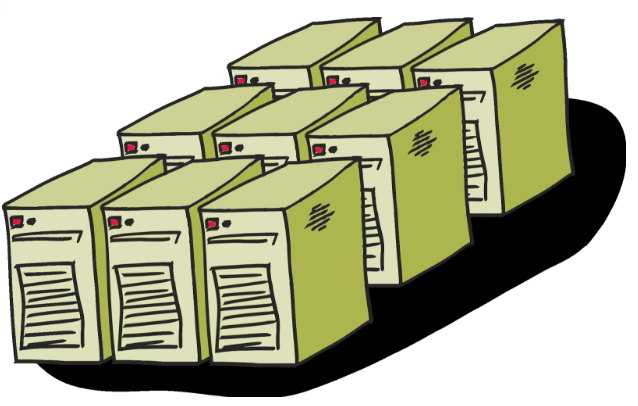
\includegraphics[width=0.8\textwidth]{./images/pcs.png}}
\end{center}
\end{frame}

\subsection{Основні відомості про Ansible}
\renewcommand\Switchsubsection{1}
\begin{frame}[fragile]
\myinsertsubsection
\begin{itemize}
    \item ``{\bf configuration management tool}'': опис стану в якому повинні перебувати сервери
    \item для опису стану серверів використовується предметно-орієнтована мова програмування (англ. Domain-specific language, DSL)
    \item використовувається для деплойменту
    \item ``{\bf orchestration tool}'': може використовуватись для розбудови інфраструктури \\ \vspace{1.5mm}{\small \graytext{ми використовуємо Terraform}}
    \item використовується для ``{\bf provisioning}'' нових серверів \\ \vspace{1.5mm}{\small\graytext{розгортання нових віртуальних машин у хмарних середовищах: EC2, Azure, Digital Ocean, Google Compute Engine, Linode і Rackspace, а також будь-які хмарні середовища, що підтримують OpenStack API}}
    \item написаний на пайтоні
    \item інші configuration management toolses: {\bf Chef}, {\bf Puppet}, {\bf SaltStack} \\
    \vspace{1.5mm}{\small\graytext{Ansible: \href{https://www.slideshare.net/JesseKeating/ansiblefest-rax}{Rackspace}\\ Chef: \href{http://www.theregister.co.uk/2013/02/04/opscode_chef_11_control_freak/}{Facebook} \\ Puppet: \href{http://puppetlabs.com/about/customers}{Several} \\ SaltStack: \href{http://aftertheclouds.altervista.org/blog/saltstack-aims-to-simplify-devops-work-with-python-configuration-management/}{LinkedIn}}}
\end{itemize}

див: https://www.infoq.com/articles/taste-test-book-review \\
Сказати, чим відрізнється від cheef і Puppet і на наступному слайді дати діаграмку.

\end{frame}

\subsection{Як працювати з Ansible}
\begin{frame}[label=none]
%
\myinsertsubsection

\begin{enumerate}
\item встановлення: sudo dnf install ansible
\item Пишеться playbook, yaml-файл
він визначає стан, в якому має бути в кінцевому випадку віддалена машина
\item в плейбуці задано віддалені машиши, які будуть конфігуруватися
\item плейбук поділено на задачі (tasks) які будуть почерзі виконуватися
\item запуск: ansible-playbook webservers.yml
\end{enumerate}

Як працює:
Ansible will make SSH connections
не потребує агента! + нема сервера.

найпростіша задача:

- name: install nginx
  dnf: name=nginx
Ansible will:
1. Generate a Python script that installs the nginx package.
2. Copy the script to web1, web2, and web3.
3. Execute the script on web1, web2, web3.
4. Wait for the script to complete execution on all hosts.
Ansible will then move to the next task in the list, and go through these same four
steps. It’s important to note that:
• Ansible runs each task in parallel across all hosts.
• Ansible waits until all hosts have completed a task before moving to the next task.
• Ansible runs the tasks in the order that you specify them.

можна дати картинку.

\end{frame}
%++++++++++++++++++++++++++++++++++++++++
\begin{frame}[plain,c,label=thanks]
\begin{center}
\textrm{\bluetext{\Large ДЯКУЮ ЗА УВАГУ}}
\end{center}
\end{frame}
\end{document}
